\documentclass[12pt]{article}  % Document class, 'article' is a good choice for beginner papers

% Basic packages for mathematical typesetting
\usepackage{amsmath}   % Essential package for mathematical symbols and environments
\usepackage{amssymb}   % Provides additional symbols like \mathbb{R}, \mathbb{N}, etc.
\usepackage{amsfonts}  % Fonts for mathematical symbols
\usepackage{graphicx}  % For including images or diagrams
\usepackage{hyperref}  % For clickable references and links
\usepackage{geometry}  % Set page margins easily
\usepackage{fancyhdr}  % Custom header/footer
\usepackage{enumerate} % For customizable lists (numbered, bullet points)
\usepackage{datetime}
\usepackage{enumitem}


% Page and margin setup
\geometry{top=1in, bottom=1in, left=1in, right=1in}  % Adjust the margins of the page
\setlength{\parskip}{1ex plus 0.5ex minus 0.5ex}  % Add space between paragraphs
\setlength{\parindent}{0pt}  % Disable paragraph indentation

% Custom commands for frequently used mathematical symbols
\newcommand{\R}{\mathbb{R}}  % Real numbers symbol
\newcommand{\N}{\mathbb{N}}  % Natural numbers symbol
\newcommand{\Z}{\mathbb{Z}}  % Integers symbol
\newcommand{\Q}{\mathbb{Q}}  % Rational numbers symbol
\newcommand{\C}{\mathbb{C}}  % Complex numbers symbol

% Theorem, Definition, and Proof environments
\newtheorem{theorem}{Theorem}[section]   % Theorem numbering by section
\newtheorem{definition}[theorem]{Definition}  % Definition with the same numbering as Theorem
\newtheorem{example}[theorem]{Example}      % Example environment
\newtheorem{remark}[theorem]{Remark}        % Remark environment

\setlist[enumerate,1]{label=\arabic*.,ref=\arabic*}
\setlist[enumerate,2]{label=\arabic{enumi}.\arabic*.,ref=\arabic{enumi}.\arabic*}


\newcommand{\notetitle}{}

% Header/footer setup
\pagestyle{fancy}
\fancyhf{}
\fancyhead[L]{Garrett Moore}
\fancyhead[C]{\notetitle}
\fancyhead[R]{\today}


\begin{document}

\clearpage
\renewcommand{\notetitle}{Table of Contents}
\label{toc}
\begin{enumerate}

\item The-Axiom-of-Completeness
\begin{enumerate}
\item \hyperref[202501180703]{Initial Definition for R}
\item \hyperref[202501180727]{Axiom of Completeness}
\item \hyperref[202501180734]{Upper and Lower Bounds}
\item \hyperref[202501180743]{Supremum and Infimum}
\item \hyperref[202501181241]{Maximum and Minimum}
\item \hyperref[202501181257]{Q and the Axiom of Completeness}
\end{enumerate}
\end{enumerate}

\newpage


\clearpage
\phantomsection
\label{202501120904}
\renewcommand{\notetitle}{Question 1}

\section*{Note Information}
\begin{itemize}
  \item \textbf{ID:} \texttt{202501120904}
  \item \textbf{Timestamp:} \texttt{\today \ \currenttime}
  \item \textbf{Tags:} \texttt{Tutoring, Chhean, Session-1}
  \item \textbf{References:}
    \begin{itemize}
      \item \href{}{}
    \end{itemize}
\end{itemize}


\section*{Main Content}
\textbf{Main Idea}\\
Suppose a particle is moving on the $x$-axis in a simple harmonic motion. Its velocity, in meters per second, at time $t$, for $0 \leq t \leq 100$ seconds, is given by $v(t) = -\frac{5}{3} \sin(\frac{t}{3})$.
The total distance traveled by the particle in the time interval $0 \leq t \leq 21 \pi$ seconds is 70 meters.\\

\textbf{Explanation}\\
The velocity of the particle is modeled by $v(t) = -\frac{5}{3} \sin (\frac{t}{3})$. 
The total distance the particle travels in the time interval $0 \leq t \leq 21 \pi$ is equal to $\int_{0}^{21 \pi} | v(t) | dt$, where $| v(t) | = \frac{5}{3} | \sin (\frac{t}{3}) |$. 
Since $\sin(\frac{t}{3}) = 0$ when $t = 3 n \pi$ for all integers $n$, the velocity function maintains its sign throughout the interval $[3 n \pi, 3(n+1) \pi]$. 
The period for the velocity function is $6 \pi$, thus twice the aforementioned interval is equal to the full period. 
This relationship can be modeled through the following expressions:
\begin{align*}
  \frac{5}{3} \int_0^{6\pi} | \sin (\frac{t}{3}) | dt &= \frac{5}{3} \cdot 2 \int_0^{3\pi} \sin (\frac{t}{3}) dt\\
                                                      &= \frac{5}{3} \cdot 2[-3 \cos(\frac{t}{3})]_0^(3\pi)\\
                                                      &= \frac{5}{3} \cdot 2[6]\\
                                                      &= 20
\end{align*}
The interval from 0 to $21 \pi$ is equal to 3.5 periods. Therefore, the total distance traveled by the particle is equal to
\begin{align*}
  3 \cdot 20 + \frac{5}{3} \cdot 6 &= 70 \text{ meters}
\end{align*}

\section*{Review}
\begin{enumerate}
  \item 
\end{enumerate}


\section*{Links to Other Notes}
\begin{itemize}
  \item \hyperref[]{}
\end{itemize}

\section*{Table of Contents}

\begin{itemize}
  \item \hyperref[toc]{TOC}
\end{itemize}


\clearpage
\phantomsection
\label{202501121340}
\renewcommand{\notetitle}{Question 2}

\section*{Note Information}
\begin{itemize}
  \item \textbf{ID:} \texttt{202501121340}
  \item \textbf{Timestamp:} \texttt{\today \ \currenttime}
  \item \textbf{Tags:} \texttt{Tutoring, Chhean, Session-1}
  \item \textbf{References:}
    \begin{itemize}
      \item \href{}{}
    \end{itemize}
\end{itemize}


\section*{Main Content}
\textbf{Main Idea}\\
Suppose a particle is moving on the $x$-axis between the time $t=0$ seconds and $t = 9$ seconds. Its initial position at $t=0$ seconds is $x(0)=2$ meters. 
The velocity-time graph of the motion is shown below.\\
\begin{center}
  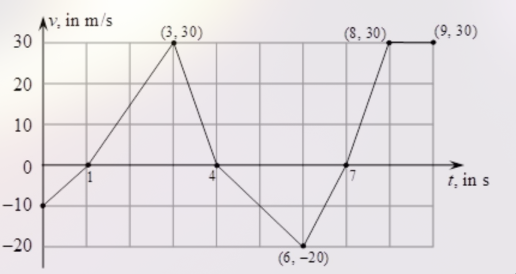
\includegraphics[width=0.5\textwidth]{Figures/Question-2.png}\\
\end{center}
On the $x$-axis, the abscissa of the farthest point to the right of the origin that the particle reaches over the time interval $0 \leq t \leq 9$ seconds is 42 meters.
\textbf{Explanation}\\
By looking at the graph, we notice that the velocity is positive on the intervals $1 \leq t \leq 4$ and $7 \leq t \leq 9$. The velocity is negative on the intervals $0 \leq t \leq 1$ and $4 \leq t \leq 7$.
The area under the curve between $t = 1$ and $t=4$ is calculated by finding the area of the triangle with base 3 and height 30:
\begin{align*}
  A_1 &= \frac{1}{2} \cdot 3 \cdot 30 = 45
\end{align*}
The area under the curve for the other three intervals are computed in a similar way below:
\begin{align*}
  A_2 &= \frac{1}{2} \cdot 1 \cdot 30 + 1 \cdot 30 = 30\\
  A_3 &= \frac{1}{2} \cdot 1 \cdot 10 = 5\\
  A_4 &= \frac{1}{2} \cdot 3 \cdot 20 = 30\\
\end{align*}
Using the areas above, we can compute $x(t)$ at key times, using the fact that $x(t) = x(0) + \int_0^t v(t) dt$:\\
At $t=1$:
\begin{align*}
  x(1) &= x(0) - A_3 = 2 - 5 = -3\\
\end{align*}
At $t = 4$:
\begin{align*}
  x(4) &= x(1) + A_1 = -3 + 45 = 42\\
\end{align*}
At $t = 7$:
\begin{align*}
  x(7) &= x(4) - A_4 = 42 - 30 = 12\\
\end{align*}
At $t = 9$:
\begin{align*}
  x(9) &= x(7) - A_2 = 12 + 30 = 42\\
\end{align*}
The particle is farthest to the right at $t = 4$ and $t = 9$, where:
\begin{align*}
  x_{max} = 42 \text{ meters}
\end{align*}

\section*{Review}
\begin{enumerate}
  \item 
\end{enumerate}


\section*{Links to Other Notes}
\begin{itemize}
  \item \hyperref[]{}
\end{itemize}

\section*{Table of Contents}

\begin{itemize}
  \item \hyperref[toc]{TOC}
\end{itemize}


\clearpage
\phantomsection
\label{202501121522}
\renewcommand{\notetitle}{Question-3}

\section*{Note Information}
\begin{itemize}
  \item \textbf{ID:} \texttt{202501121522}
  \item \textbf{Timestamp:} \texttt{\today \ \currenttime}
  \item \textbf{Tags:} \texttt{Tutoring, Chhean, Session-1}
  \item \textbf{References:}
    \begin{itemize}
      \item \href{}{}
    \end{itemize}
\end{itemize}


\section*{Main Content}
\textbf{Main Idea}\\
The velocity-time graph of a particle moving along a straight line is shown below. Time $t$ is measured in minutes, and the velocity $v(t)$ is measured in meters per minute.
\begin{center}
  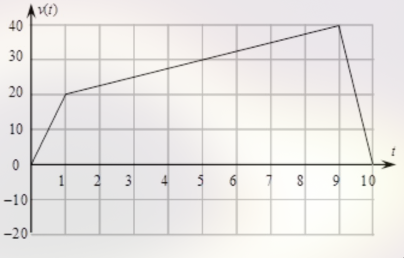
\includegraphics[width=0.5\textwidth]{Figures/Question-3.png}
\end{center}
If the average acceleration of the particle in the time interval $1 \leq t \leq 9$ minutes is $k$ m/min$^2$, the value of $k$ is .\\
\textbf{Explanation}\\
The average acceleartion can be calculated using the following formula:
\begin{align*}
  k = \frac{\delta v}{\delta t}\\ 
\end{align*}
According to the graph, $\delta v = v(9) - v(1) = 40-20 = 20$. Thus,
\begin{align*}
  k = \frac{20}{8} = \frac{5}{2} = 2.5 \text{ m / min}^2
\end{align*}


\section*{Review}
\begin{enumerate}
  \item 
\end{enumerate}


\section*{Links to Other Notes}
\begin{itemize}
  \item \hyperref[]{}
\end{itemize}

\section*{Table of Contents}

\begin{itemize}
  \item \hyperref[toc]{TOC}
\end{itemize}


\clearpage
\phantomsection
\label{202501121636}
\renewcommand{\notetitle}{Question-4}

\section*{Note Information}
\begin{itemize}
  \item \textbf{ID:} \texttt{202501121636}
  \item \textbf{Timestamp:} \texttt{\today \ \currenttime}
  \item \textbf{Tags:} \texttt{Tutoring, Chhean, Session-1}
  \item \textbf{References:}
    \begin{itemize}
      \item \href{}{}
    \end{itemize}
\end{itemize}


\section*{Main Content}
\textbf{Main Idea}\\
Suppose a cylindrical reservoir of radius 4 meters is being filled with water. The rate at which the level of water is increasing is given by $u(t) = 8 - 2 \sin (\frac{\pi t}{18})$ meter per minute.
The rate at which the volume of water in the reservoir is increasing at $t = 9$ minutes is $ \pi$ cubic meters per minute.\\

\textbf{Explanation}\\
The volume of water in a cylindrical reservoir is given by:
\begin{align*}
  V = \pi r^2 h,\\
\end{align*}
where $r = 4$ and $h$ is the water level in the reservoir. 
The rate of change of the volume is related to the rate of change of the water level by:
\begin{align*}
  \frac{dV}{dt} &= \pi r^2 \frac{dh}{dt}\\
  &= 16 \pi (8 - 2 \sin(\frac{\pi t}{18}))\\
\end{align*}
At $t = 9$:
\begin{align*}
  \frac{dV}{dt} &= 16 \pi (8 - 2 \sin (\frac{\pi (9)}{18}))\\
                &= 16 \pi (6)\\
                &= 96 \pi \text{ cubic meters per minute}
\end{align*}

\section*{Review}
\begin{enumerate}
  \item 
\end{enumerate}


\section*{Links to Other Notes}
\begin{itemize}
  \item \hyperref[]{}
\end{itemize}

\section*{Table of Contents}

\begin{itemize}
  \item \hyperref[toc]{TOC}
\end{itemize}


\clearpage
\phantomsection
\label{202501121712}
\renewcommand{\notetitle}{Question 5}

\section*{Note Information}
\begin{itemize}
  \item \textbf{ID:} \texttt{202501121712}
  \item \textbf{Timestamp:} \texttt{\today \ \currenttime}
  \item \textbf{Tags:} \texttt{Tutoring, Chhean, Session-1}
  \item \textbf{References:}
    \begin{itemize}
      \item \href{}{}
    \end{itemize}
\end{itemize}


\section*{Main Content}
\textbf{Main Idea}\\
Suppose, for $0 \leq t \leq 20$ hours, water is being pumped into a reservoir at the rate of $R(t) = \frac{1}{3}t^2 - t + 2$ cubic meters per hour and removed from the reservoir at the rate of $r(t) = 2t + 14$ cubic meters per hour.
If the amount of water in the reservoir is increasing during the time interval $(a,20)$ and decreasing elsewhere, the value of $a$ is 12.\\

\textbf{Explanation}\\
To find the time interval in which the amount of water in the reservoir is increasing, we set up the following inequality:
\begin{align*}
  R(t) - r(t) > 0.\\
\end{align*}
We only care about the critical point in which the net rate of change switches sign, thus we need to solve:
\begin{align*}
  R(t) - r(t) = 0.\\
\end{align*}
The net rate of change is equal to $\frac{1}{3}t^2 - 3t - 12$. Setting this expression equal to 0 and solving gives us:
\begin{align*}
  \frac{1}{3}t^2 - 3t - 12 &= 0\\
  t^2 - 9t - 36 &= 0\\
  (t - 12)(t + 3) &= 0\\
  t &= 12, -3\\
\end{align*}
Since $t = -3$ is not within the inteval $0 \leq t \leq 20$, $a = 12$.\\

\section*{Review}
\begin{enumerate}
  \item 
\end{enumerate}


\section*{Links to Other Notes}
\begin{itemize}
  \item \hyperref[]{}
\end{itemize}

\section*{Table of Contents}

\begin{itemize}
  \item \hyperref[toc]{TOC}
\end{itemize}


\clearpage
\phantomsection
\label{202501121828}
\renewcommand{\notetitle}{Question 6}

\section*{Note Information}
\begin{itemize}
  \item \textbf{ID:} \texttt{202501121828}
  \item \textbf{Timestamp:} \texttt{\today \ \currenttime}
  \item \textbf{Tags:} \texttt{Tutoring, Chhean, Session-1}
  \item \textbf{References:}
    \begin{itemize}
      \item \href{}{}
    \end{itemize}
\end{itemize}


\section*{Main Content}
\textbf{Main Idea}\\
 The velocity-time graph of a particle moving on a straight line is shown below. Time $t$ is measured in seconds, and the velocity $v(t)$ is measured in meters per second.
 \begin{center}
  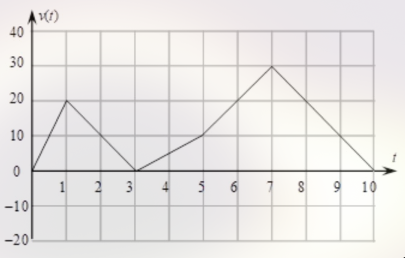
\includegraphics[width=0.5\textwidth]{Figures/Question-6.png}
 \end{center}
 If at $t = 0$ seconds, the position of the particle is at 20 meters, then at $t = 10$ seconds, its position is at 145 meters.\\

\textbf{Explanation}\\
The velocity-time graph can be divided into 5 sections, comprised of 4 triangles and 1 rectangle. To begin, calculate the areas of these 5 sections:
\begin{align*}
  A_1 &= \frac{1}{2} \cdot 3 \cdot 20 = 30\\
  A_2 &= \frac{1}{2} \cdot 2 \cdot 10 = 10\\
  A_3 &= \frac{1}{2} \cdot 4 \cdot 20 = 40\\
  A_4 &= \frac{1}{2} \cdot 1 \cdot 10 = 5\\
  A_5 &= 4 \cdot 10 = 40\\
\end{align*}
The total distance can be modeled by the following expression:
\begin{align*}
  x(0) + \int_0^t v(t) dt.
\end{align*}
Given that $x(0) = 20$ and $\int_0^t v(t) dt = A_1 + A_2 + A_3 + A_4 + A_5 = 125$, at $t = 10$:
\begin{align*}
  x(10) &= 20 + 125 = 145 \text{ meters}.\\
\end{align*}


\section*{Review}
\begin{enumerate}
  \item 
\end{enumerate}


\section*{Links to Other Notes}
\begin{itemize}
  \item \hyperref[]{}
\end{itemize}

\section*{Table of Contents}

\begin{itemize}
  \item \hyperref[toc]{TOC}
\end{itemize}


\end{document}
